\section{Linear Regression (LR)}
%%%%%%%%%%%%%%%%%%%%%%%%%%%%%%%%
Linear regression is widely used because it is a method which is easy to calculate. Also, linear models are easy to interpret and therefore chosen in many different contexts. However, it is important to remember the underlying assumptions when using LR.
\subsection{Assumptions}\label{sec:ass}
	\begin{exmp}[Linear and non-linear models]{exmp:lin}
		Which of the following models is linear?
		\begin{enumerate}
			\item $y=\alpha_0+\alpha_1 x_1^2+\alpha_2 x_2 + \alpha_3 x_3 + \epsilon$
			\item $y=\alpha x_1^\beta \mu x_2^\gamma$
			\item $y=\alpha_0+\alpha_1 x_1+\alpha_2 x_2 + \eta$
			\item $y=\alpha+\frac{tan\left(\beta x_1 + \gamma x_2^2\right)}{1+2 x_1^3} + \epsilon$
		\end{enumerate}
		Solution:
		\begin{enumerate}
			\item Is linear because all parameters $\alpha$ are linear, the regressors $x$ can be transformed. $\epsilon$ is an error term.
			\item Is non-linear, but can be transformed to a linear model by an easy logarithmic (ln) transformation.
			\item Is linear.
			\item Is non-linear because the parameters are in non-linear form which cannot easily be transformed to a linear function.
		\end{enumerate}		
	\end{exmp}
	\subsubsection{Linearity in the unknown parameters (A1)}\label{sec:ass1}
		The unknown parameters linking the dependent variable $y$ with the known explanatory variables or regressors $x$ have to be linear.  
		\begin{equation*}
			\overbrace{y}^{\hbox{dependent}}_{n\times 1}=\overbrace{x}^{\hbox{regressor}}_{n\times k}\times\overbrace{\beta}^{\hbox{parameter}}_{k\times 1}+\overbrace{\epsilon}^{\hbox{error}}_{n\times 1}
		\end{equation*}
		Where $n=[1,2,...,n]$ is the sample size and $\beta=[0,1,...,k-1]$ are the number parameters we are looking for.
		\begin{align*}
			\begin{cases}
				y_1&=\beta_0+\beta_1 x_{11}+\beta_2 x_{12}+\cdots+\beta_{k-1} x_{1k-1}+\epsilon_1\\
				&\vdots\\
				y_n&=\beta_0+\beta_1 x_{n1}+\beta_2 x_{n2}+\cdots+\beta_{k-1} x_{nk-1}+\epsilon_n
			\end{cases}			
		\end{align*}
	\subsubsection{Unbiasedness of the error term (A2)}		
		The error term consists of random errors and variables that have been excluded in an act of simplifying. However, the error term shall not have any systematic bias but be independently and identically distributed (i.i.d.) for all $\epsilon_i\sim(0,\sigma^2)$ with mean 0 (unbiased) and an unknown variance. This implies that $E(\epsilon_i)=0$.	
	\subsubsection{Homoscedasticity of the error term (A3)}		
		The distribution has the variance $var(\epsilon_i)=\sigma^2 $.	This variance is the same for all observations.
	\subsubsection{Independence of the error term (A4)}	
		The errors of different observations are not related: $cov(\epsilon_i,\epsilon_j)=0\;\forall\;i\neq j$.
	\subsubsection{Exogeneity of the regressors (A5)}
		The values of the explanatory variables or regressors are determined solely by influences \emph{outside} of the environment depicted by the model. This means, $y$ shall not have any direct influence on the value of any $x$.
		\begin{equation*}
			\forall\;(i,j)\varepsilon\left\{0,...,k-1\right\}\times\left\{1,...,n\right\},\quad cov(x_i,\epsilon_j)=0
		\end{equation*}
	\subsubsection{Normal distribution of error terms (A6)}\label{sec:ass6}
		For the purpose of testing the model, we also require the error terms $\epsilon_i$ to be approximately normal distributed.
		\begin{equation*}
			\forall\;(i)\varepsilon\left\{1,...,n\right\},\quad \epsilon_i\sim N(0,\sigma^2)
		\end{equation*}																	
	
	From these assumption we can conclude:
	\begin{equation*}
		y_i\sim N\left((x)_i\beta,\sigma^2\right)
	\end{equation*}
	with $(x)_i$ as the $i^{th}$ row (dimension $1\times k$) of the regressors $x$ and $\beta$ with  dimension $k\times 1$. This means, we assume all $x_{ij}$ are known.
\subsection{Estimation}
	To find estimates for the unknown $\beta$ and $\sigma^2$, we use the method of \emph{linear regression}. It helps to understand how the regressors $x$ affect the dependent variable $y$.	
	\subsubsection{Least Squares}\label{sec:ols}
		\begin{fig}[Ordinary least squares]{fig:ols}{h}
			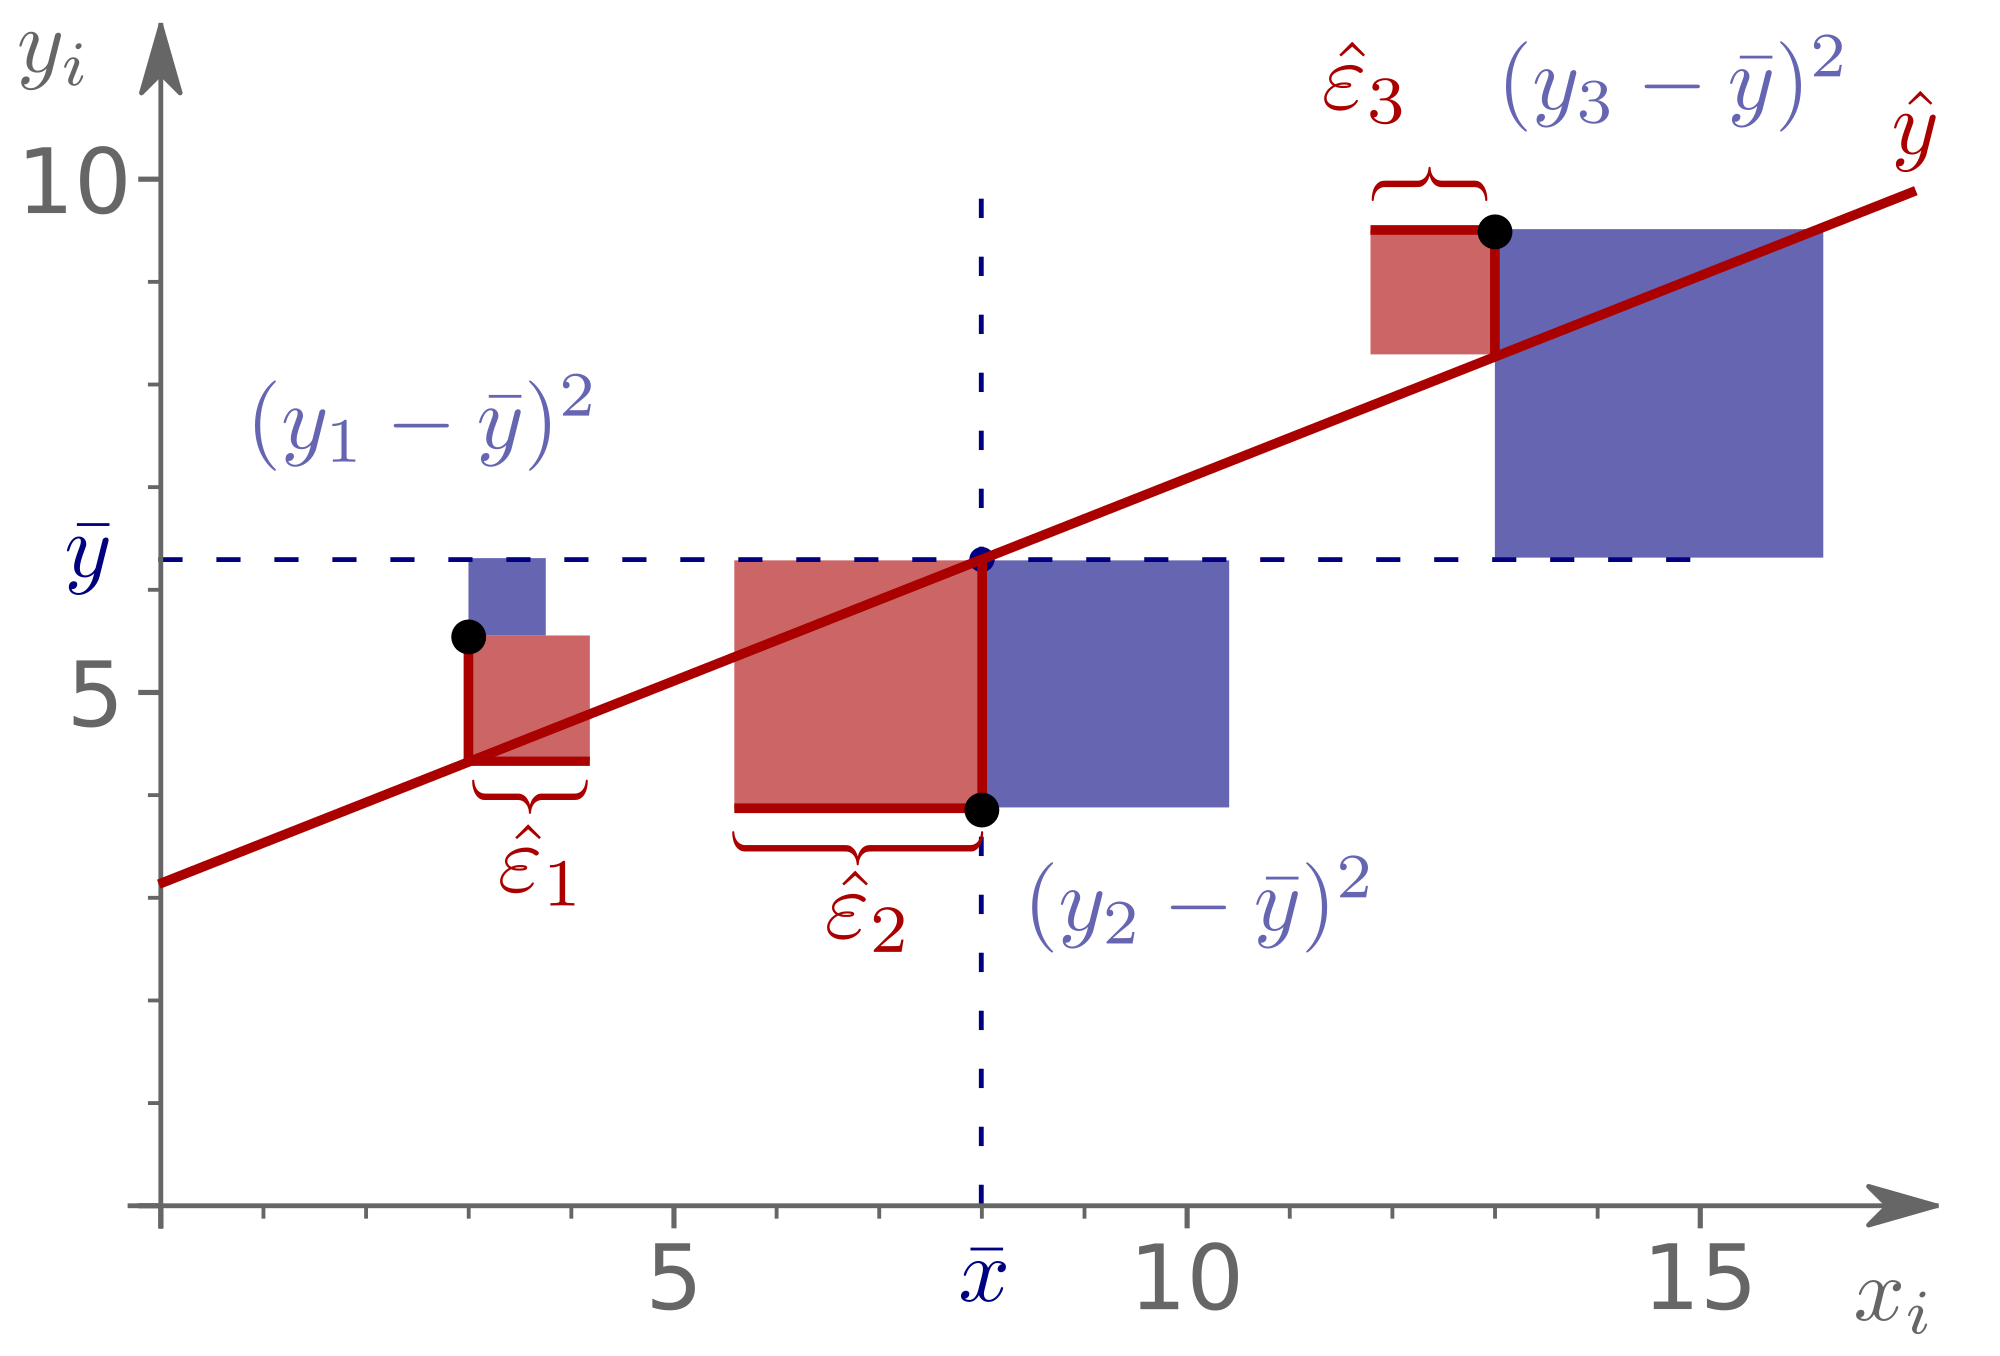
\includegraphics[width=\textwidth]{P17ols.png}	
			\credits{By Debenben at Wikipedia Commons. CC BY-SA 4.0.}											
		\end{fig}	
		The \emph{method of least squares}, also known as ordinary least squares (OLS), is one of the most common estimations used in linear regression. The method tries to draw the best fitting straight line into the datapoints $(x_n,y_n)$. By minimizing sum of the square of the distance between the line and each datapoint (the error or residuum), we will get the \emph{BLUE}, the best linear unbiased estimator.
		\begin{equation*}
			\min_{\beta_0,...,\beta_{k-1}} \sum\limits_{i=1}^n \left(y_i-\hat{y_i}\right)^2
		\end{equation*}
		This means, seeing this as a function $f(\beta_0,\beta_1,...\beta_{k-1})$ stating the sum of the squares of the differences between observed and estimated values, we are trying to minimize this function. With $\beta_0$ as a constant intercept, we can define $x_0\equiv 1$.
		\begin{equation*}
		\min_{\beta_0,...,\beta_{k-1}} f(\beta_0,\beta_1,...\beta_{k-1}) = \min_{\beta_0,...,\beta_{k-1}} \sum\limits_{i=1}^n \left(y_i-\hat{y_i}\right)^2 = \min_{\beta_0,...,\beta_{k-1}}  \sum\limits_{i=1}^n \left(y_i-\sum\limits_{j=0}^{k-1}\beta_j x_{ji} \right)^2
		\end{equation*}
		To find estimates of  $\beta_0,\beta_1,...\beta_{k-1}$ we find the derivative:
		\begin{equation*}
			\frac{\partial f(\cdot)}{\partial \beta_j}\quad\text{for }j\varepsilon\{0,1,...,k-1\}
		\end{equation*}
		\begin{align*}
				\frac{\partial f(\cdot)}{\partial \beta_0}&=\sum\limits_{i=1}^n -2\left(y_i-\sum\limits_{j=0}^{k-1}\beta_j x_{ji}\right)\qquad\text{(1)}\\
				&\vdots\\
				\frac{\partial f(\cdot)}{\partial \beta_j}&=\sum\limits_{i=1}^n -2\left(y_i-\sum\limits_{j=0}^{k-1}\beta_j x_{ji}\right)\qquad\text{(j)}\\				
		\end{align*}
		This means, $k$ equations for $k$ unknown $\beta$, so we can solve this. In matrix notation with $X$ as the matrix of explanatory observations, the solution will be (according to the method shown in appendix \ref{app:der}):
		\begin{equation*}
			\hat{\beta}=(X'X)^{-1}X'Y
		\end{equation*}
		From equation (1), we have
		\begin{equation*}
			 \sum\limits_{i=1}^n y_i-\sum\limits_{j=0}^{k-1}\beta_j   \sum\limits_{i=1}^n x_{ji}=0.
		\end{equation*}
		Dividing by $n$ gives us
		\begin{equation*}
			\underbrace{\frac{1}{n}\sum\limits_{i=1}^n y_{i}}_{=\bar{y}}-\sum\limits_{j=0}^{k-1}\beta_j \underbrace{\frac{1}{n}\sum\limits_{i=1}^n x_{ji}}_{=\bar{x}}=0
		\end{equation*}	
		\begin{equation*}
			\Longrightarrow \bar{y}=\sum\limits_{j=0}^{k-1}\hat{\beta_j}\bar{x_j}.
		\end{equation*}
		In other words, the regression line goes through the sample mean.
\subsubsection{Maximum Likelihood}
	The idea of this method is to \emph{maximize the likelihood} or chance of getting our sample when observing a population. This means to puck a parametric family and find the parameters that maximize the chance of observing the sample. Recall, assumptions A1-A6 (\ref{sec:ass}): $y_i\sim N\left((x)_i\beta,\sigma^2\right)$. Let $f(\cdot)$ designate the joint distribution of $\{y_1,y_2,...,y_n\}$.
	
	But we assumed that the error terms $\epsilon$ (and therefore $y_1,y_2,...,y_n$) are from a random sample and thus i.i.d. In consequence, the joint density of $y_1,y_2,...,y_n$ is equal to the products of the marginal densities of $y_1,y_2,...,y_n$.
	\begin{exmp}[Density of a normal distribution]{exmp:normdens}
		$W$ is normally distributed: $W\sim N(\mu,\sigma^2)$. Then, the density of $W$ is:
		\begin{equation*}
			f(w)=\frac{1}{\sqrt{2\pi\sigma^2}}\,exp\left[-\frac{1}{2}\left(\frac{w-\mu}{\sigma}\right)^2\right]
		\end{equation*}
	\end{exmp}
	In consequence, the joint density of $y_1,y_2,...,y_n$ is:
	\begin{equation*}
		f(y,x,\beta,\sigma^2)=\prod_{i=1}^{n}\frac{1}{\sqrt{2\pi\sigma^2}}\,exp\left[-\frac{1}{2}\left(\frac{y_i-\sum\limits_{j=0}^{k-1}\beta_j x_{ij}}{\sigma}\right)^2\right]
	\end{equation*}
	$f(\cdot)$ is a product of small values (all factors in the product are $\leq 1$). This makes exact calculations hard. Also, taking the derivative for maximizing the function is less convenient with a product function than with a sum. So before maximizing the function, we perform a logarithmic transformation. The log-likelihood function then is as follows:
	\begin{align*}
		\mathcal{L}(\beta,\sigma^2|y,x)&=ln\left(\prod_{i=1}^{n}\frac{1}{\sqrt{2\pi\sigma^2}}\,exp\left[-\frac{1}{2}\left(\frac{y_i-\sum\limits_{j=0}^{k-1}\beta_j x_{ij}}{\sigma}\right)^2\right]\right)\\
		&=-\frac{n}{2}ln(2\pi)-\frac{n}{2}ln(\sigma^2)-\frac{1}{2\sigma^2}\sum\limits_{i=1}^n\left(y_i-\sum\limits_{j=0}^{k-1}\beta_j x_{ij}\right)^2\\
		\frac{\partial\mathcal{L}}{\partial\sigma^2}&=0-\frac{n}{2}\frac{1}{\sigma^2}+\frac{1}{2\sigma^4}\sum\limits^n_{i=1}\left(y_i-\sum\limits_{j=0}^{k-1}\beta_j x_{ij}\right)^2\\
		\Longrightarrow \hat{\sigma}^2&=\frac{1}{n}\sum\limits_{i=1}^n(			\underbrace{y_i-\hat{y_i}}_{=\hat{\epsilon_i}})^2\\
		&=\frac{1}{n}\sum\limits_{i=1}^n \hat{\epsilon_i}=\frac{1}{n}\sum\limits_{i=1}^n \left(\hat{\epsilon_i}-E(\hat{\epsilon_i})\right)^2
	\end{align*}
	With $E(\hat{\epsilon_i})=0$. This expression is similar to calculating the variance as seen in definition \ref{defi:variance}. In this sense, we can see it as the variance of the error. Let us write $\mathcal{L}$ as follows:
	\begin{align*}
		\mathcal{L}&=-\frac{n}{2}ln(2\pi)-\frac{n}{2}ln(\sigma^2)-\frac{1}{2\sigma^2}\underbrace{(Y-X\beta)'}_{\hbox{row}}\underbrace{(Y-X\beta)}_{\hbox{column}}\\
		&=-\frac{n}{2}ln(2\pi)-\frac{n}{2}ln(\sigma^2)-\frac{1}{2\sigma^2}\sum\limits_{i=1}^n \left(y_i - \sum\limits_{j=0}^{k-1} \beta_j x_{ij} \right)^2\\
		\frac{\partial\mathcal{L}}{\partial\sigma^2}&=\frac{1}{n}\sum\limits_{i=1}^n \hat{\epsilon}_i,\qquad\text{Recall: }E(\epsilon_i)=0\\
		\frac{\partial\mathcal{L}}{\partial\beta}&=0+0-\frac{1}{2\sigma^2}\frac{\partial}{\partial\beta}\left[y'y-y'x\beta-\beta'x'y+\beta\right]\\
		&=-\frac{1}{2\sigma^2}\left[0-2x'y+2x'x\beta\right]\\
		\text{Recall: }G(\beta)&=\beta' M \beta,\quad \frac{\partial G}{\partial\beta}=M'\beta+M\beta\\
		(x'x)'&=x'x''=x'x\\
		\text{With symmetry }M&=M'\\
		M'\beta+M\beta&=2M\beta\\
		\frac{\partial\mathcal{L}}{\partial\beta}&=0\Longrightarrow\left[x'y=(x'x)\beta\right]\\
		\Longrightarrow\hat{\beta}&=(x'x)^{-1}x'y\\
		\text{Provided }rank(x'x)&=k\quad (x'x \text{ has an inverse})
	\end{align*}
\subsubsection{Properties of OLS \& ML estimators}
	\myparagraph{Expected value}
		\begin{align*}
			E(\hat{\beta})&=E\left((x'x)^{-1}x'y\right)=(x'x)^{-1}x'E(y)\\ %%x'xx is known and non-random (A5),y is N(x \beta, \sigma^2 I)
			%from a2: y=x\beta+\epsilon = x\beta
			\text{With }x\text{ as a known an non-random variable}
			E(\hat{\beta})&=(x'x)^{-1}x'x\beta=\beta\\
			E(\hat{\beta})&=\beta
		\end{align*}
		This means, $\hat{\beta}$ is an unbiased estimator.
	\myparagraph{Variance}
		\begin{align*}
			\hat{\beta}&=(x'x)^{-1}x'y=(x'x)^{-1}x'(X\beta+\epsilon)\\
			&=(x'x)^{-1}x'x\beta+(x'x)^{-1}x'\epsilon\\
			&=\beta+(x'x)^{-1}x'\epsilon\\
			\text{Recall: Let W be a random variance. Then: }\\
			var(W)&=E\left((W-E(W))^2\right)\\
			var(\hat{\beta})&=E\left((\hat{\beta}-\beta)(\hat{\beta}-\beta)'\right)\\
			&=E\left((x'x)^{-1}x'\epsilon\epsilon'x(x'x)^{-1}\right)\\
			&=(x'x)^{-1}x'E(\epsilon\epsilon')x(x'x)^{-1}\\
			&=(x'x)^{-1}x'\sigma^2 I_n x(x'x)^{-1}\\
			&=\sigma^2 (x'x)^{-1}x'x(x'x)^-1=\sigma^2(x'x)^{-1},\,(x'x)^{-1}x'x=I_k\\
			var(\hat{\beta})&=\sigma^2(x'x)^{-1}\\
			\widehat{var(\hat{\beta})}&=\hat{\sigma^2}(x'x)^{-1}\\
			\hat{\beta}&=\begin{pmatrix}
				\hat{\beta}_0\\
				\hat{\beta}_1\\
				\vdots\\
				\hat{\beta}_{k-1}
			\end{pmatrix}
		\end{align*}
		The standard error is the square root of the variance.
		\begin{gather*}
			SE(\hat{\beta}_j)=\sqrt{\hat{\sigma^2}(x'x)^{-1}_{jj}}\\
			var(\hat{\beta})=\begin{pmatrix}
				var(\hat{\beta}_0)&cov(\hat{\beta}_0,\hat{\beta}_1)&\cdots&cov(\hat{\beta}_0,\hat{\beta}_{k-1})\\
				cov(\hat{\beta}_1,\hat{\beta}_0)&var(\hat{\beta}_1)&\cdots&cov(\hat{\beta}_1,\hat{\beta}_{k-1})\\
				\vdots&\vdots&\ddots&\vdots\\
				cov(\hat{\beta}_{k-1},\hat{\beta}_0)&cov(\hat{\beta}_{k-1},\hat{\beta}_1)&\cdots&var(\hat{\beta}_{k-1})
			\end{pmatrix}
		\end{gather*}
	\myparagraph{Gauss-Markov theorem}
		Assume that A1-A5 (\ref{sec:ass1}) hold. Then, the ML-OLS estimators achieve minimum variance in the class of linear, unbiased estimators. So, they are most efficient.
		
		\emph{Proof:} Let $\tilde{\beta}$ be another linear, unbiased estimator. Without loss of generality, we write
		\begin{align*}
			\tilde{\beta}&=\hat{\beta}+Dy=\left[(x'x)^{-1}+D\right]y\\
			E(\tilde{\beta})&=\beta\quad(\tilde{\beta}\text{ is unbiased })\\
			E(\tilde{\beta})&=E\left(\left[(x'x)^{-1}x'+D\right]\left[x\beta+\epsilon\right]\right)\\
			&=\underbrace{(x'x)^{-1}x'x}_{I_k}\beta+Dx\beta+\left[(x'x)^{-1}x'+D\right]\underbrace{E(\epsilon)}_{=0\,(A2)}\\
			&=\beta+Dx\beta=(I+Dx)\beta=\beta\Longrightarrow Dx=0\\
			var(\tilde{\beta})&=var(Cy)=C var(y)C'=C\sigma^2 I_m C'\\
			&=\sigma^2 C C'\\
			&=\sigma^2 \left[(x'x)^{-1}x'+D\right]\left[(x'x)^{-1}x'+D'\right]\\
			&=\sigma^2 \left[(x'x)^{-1}\underbrace{x'x(x'x)^{-1}}_{I_k}+\underbrace{(x'x)^{-1}x'D'}_{=0}+D D' +\underbrace{Dx(x'x)^{-1}}_{=0}\right]\\
			&=\sigma^2(x'x)^{-1}+\sigma^2 D D'\\
			&=var(\hat{\beta})+\sigma^2 D D'
		\end{align*}
		$D D'$ is positive semi-definite, i.e. $\forall v,\,v' D D' v=(D'v)'(D'v)\geq 0$. Recall, this means that $norm(D'v)\geq 0$.	So, $var(\tilde{\beta})$ is larger than the variance $var(\hat{\beta})$. As a consequence, $\hat{\beta}$ is BLUE (\ref{sec:ols}). Linearity here means, in $y,\,\hat{\beta}=(x'x)^{-1}xy)$ with $x$ known.\begin{famo}[Carl Friedrich Gauß]{famo:gauss}
			\emph{Johann Carl Friedrich Gauß} (30 April 1777 – 23 February 1855) in Brunswick, in the Duchy of Brunswick-Wolfenbüttel (now part of Lower Saxony, Germany, as the son of poor working-class parents. \emph{Gauß was a child prodigy}. A contested story relates that, when he was eight, he figured out how to add up all the numbers from 1 to 100. 

Gauß' intellectual abilities attracted the attention of the Duke of Brunswick, who sent him to the Collegium Carolinum (1792 to 1795, and to the University of Göttingen (1795 to 1798). While there, Gauß independently rediscovered several important theorems. In 1796, he became the first to prove the quadratic reciprocity law, which allows mathematicians to \emph{determine the solvability of any quadratic equation}. He also conjectured the prime number theorem, which gives a good understanding of how prime numbers are distributed among integers. In his 1799 doctorate, Gauß proved \emph{that every nonconstant single-variable polynomial with complex coefficients has at least one complex root}.  Gauß also made important contributions to number theory in his 1801 book Disquisitiones Arithmeticae.

In 1831 Gauß developed a fruitful collaboration with physicist Wilhelm Weber, leading to new knowledge in magnetism and the \emph{discovery of Kirchhoff's electric circuit laws}. They constructed the first electromechanical telegraph in 1833, which connected the observatory with the institute for physics in Göttingen. In 1840, Gauß published his influential \enquote{Dioptrische Untersuchungen}, in which he gave the first systematic analysis on the formation of images under a paraxial approximation (\emph{Gaußian optics}).

Gauß' personal life was overshadowed by the early death of his first wife, Johanna Osthoff, in 1809, soon followed by the death of one child, which caused him to become depressed. When his second wife died in 1831 after a long illness, one of his daughters took over the household and cared for Gauß for the rest of his life. Gauß had six children, 3 with each wife. 
 
Gauß made major contributions to various areas of mathematics (including geometry and number theory) and physics (including magnetism and optics). The importance of his contributions is often compared to those of Newton. He also made some key contributions to statistics. The most important one is the development of \emph{least squares estimation recursive methods}, which he discusses in a book on planetary orbits. He also proposed some, which are used for time series analysis and were used to help calculate the trajectory of the Apollo spacecraft. He is also \emph{credited with developing the normal distribution} (also called the Gaussian distribution or bell curve), which is extremely useful in probability and statistics.
\credits{Sources: \url{https://en.wikipedia.org/wiki/Carl_Gauss}, \url{http://www.sciencedirect.com/science/article/pii/0315086078900496}}
		\end{famo}	
			
\subsubsection{Inference}
	Let us now also assume that A6 (\ref{sec:ass6}, normality of $\epsilon$) holds. Since $\hat{\beta}$ is a linear estimator (in $y$), and since $y\sim N(x\beta,\sigma^2 I_n)$ with i.i.d., then $\hat{\beta}$ as a linear combination of a independent normals is also normal distributed.
	\myparagraph{Hypothesis Testing}
		From the fact that $\hat{\beta}\sim N$,
		\begin{equation*}
			z^*=\frac{\hat{\beta}_l-\beta_{l0}}{\sigma(\hat{\beta}_l)}\sim N(0,1)
		\end{equation*}
		with $l\varepsilon\{0,1,...,k-1\}$, $\sigma(\hat{\beta}_l)$ as the standard error of $\hat{\beta}$ which is the square root of its variance. 
		
		In practice, we do not know $\sigma(\hat{\beta}_l)$. Because of that, we use
		\begin{equation*}
			T^*=\frac{\hat{\beta}_l-\beta_{l0}}{s(\hat{\beta}_l)}\text{. If $H_0$ is true, } t*\sim t(n-k)\text{ with } k=\#\text{ of }\beta\text{ in the model.}
		\end{equation*}
	\myparagraph{Confidence Interval}
			We have, given $\alpha\varepsilon(0,1)$,
			\begin{equation*}
				CI(1-\alpha)=\hat{\beta}_l\pm t_{\frac{\alpha}{2}}(n-k)\cdot s(\hat{\beta}_l)
			\end{equation*}
		\myparagraph{Joint test (f-test)}
			\emph{Step 1:}
			\begin{align*}
				H_0:\; &\beta_l=0\,\wedge\,\beta_{l+1}=0\,\wedge\,\cdots\wedge\,\beta_{k-1}=0\\
				H_1:\; &\text{not }H_0
			\end{align*}
			
			\emph{Step 2:}
			\begin{equation*}
				F^*=\frac{(SSE_R-SSE_F)/\#restrictions}{SSE_F/(n-k)}
			\end{equation*}
			with $\#restrictions=k-l$.
			If $H_0$ is true, $F^*\sim F(k-l,n-k)$.
			$SSE$ is the sum of the square errors $SSE=\sum\limits_{i=1}^n\hat{\epsilon_i^2}$.
			$R$ are parameters for the restricted model (obtained by imposing $H_0$) and $F$ of the full model with $k= \#$ of $\beta$.
			
			\begin{exmp}[Restricted linear model]{exmp:restr}
				$y_i=$ demand for bikesharing at location $i$.
				\begin{align*}
					F:\; y_i&=\beta_0+\beta_1 Inc_i +\beta_2 GenZ_i+\beta_3 GenY_i+\beta_4 GenX_i+\beta_5 Edu_i+\beta_6 Carpp_i +\epsilon_i\\
					R:\; y_i&=\beta_0+\beta_1 Inc_i +\beta_2 GenZ_i+\beta_3 GenY_i +\mu_i						
				\end{align*}
				Joint test: $H_0: \beta_4=0\,\wedge\,\beta_5=0\,\wedge\,\beta_6=0$					
			\end{exmp}
			
			\emph{Step 3:}
				\begin{enumerate}[	a.]
					\item Pick $\alpha=Pr(\text{Type I error})$,
					\item calculate $F^*_{calc}$,
					\item rejection region and locate $F^*_{calc}$, and
					\item conclude.
				\end{enumerate}
				\begin{exmp}[Testing for different values than zero]{exmp:othertests}
					Compare to the test for parameters to be zero in example \ref{exmp:restr}.
					\begin{align*}
						y_i&=\beta_0+\cdots+(1+\beta_6)Carpp_i+\epsilon_i\\
						R:\; y_i&=\beta_0+\cdots+\beta_3 GenY_i+Carpp_i+\mu_i
					\end{align*}
					Joint test: $H_0: \beta_4=0\,\wedge\,\beta_5=0\,\wedge\,\beta_6=0$
				\end{exmp}				
	\subsubsection{Goodness of Fit}
		\myparagraph{Square Errors}
			$R^2$ is the fraction of the variation of the dependent variable explained by the model. Consider $\{y_1,y_2,...,y_n\}$ as our dependent variable. One way to measure the variations of $y$ is
			\begin{equation*}
				SST=\sum\limits_{i=1}^n(y_i-\bar{y})^2
			\end{equation*}
			with $SST$ as the total sum of squares. One way to characterize how much a linear model \emph{explains} the variations of $y$ is:
			\begin{equation*}
				SSR=\sum\limits_{i=1}^n(\hat{y_i}-\bar{y})^2
			\end{equation*}
			\begin{equation*}
				R^2\equiv\frac{SSR}{SST}
			\end{equation*}
			We also can define
			\begin{equation*}
				SSE=\sum\limits_{i=1}^n \hat{\epsilon}^2_i
			\end{equation*}
			with $SSE$ as the square sum of errors and $SST=SSR+SSE$.
			\begin{align*}
				SST&=\sum\limits_{i=1}^n (y_i-\bar{y})^2=\sum\limits_{i=1}^n (y_i\hat{y}_i+\hat{y}_i-\bar{y})^2\\
				&=\sum\limits_{i=1}^n (y_i-\hat{y}_i)+2\sum\limits_{i=1}^n (y_i-\hat{y})(\hat{y}_i-\bar{y})+\sum\limits_{i=1}^n (\hat{y}_i-\bar{y})^2\\
				\sum\limits_{i=1}^n \hat{\epsilon}_i(\hat{y}_i-\bar{y})^2&=\hat{\epsilon}'\cdot(x\hat{\beta}-\bar{y}1)=\hat{\epsilon}' x\cdot \hat{\beta}-\bar{y}\hat{\epsilon}'1\\
				\hat{\epsilon}'x&=(y-\hat{y})'x=(y-x(x'x)^{-1}x'y)'x\\
				&=(y'-y'x(x'x)^{-1}x')x\\
				&=y'(x-x(x'x)^{-1}x'x)=y'(x-x)=0\\
				\hat{\epsilon}'1&=\sum\limits_{i=1}^n=\hat{\epsilon}_i=0
			\end{align*}
			because $E(\epsilon)=0$ which comes from $\frac{\partial \mathcal{L}}{\partial\beta_0}=0$.
			In consequence,
			\begin{align*}
				SST&=SSR+SSE\\
				R^2&=\frac{SSR}{SST}\\
				SSR,SST,SSE&\geq 1\\
				\Longrightarrow 0\leq R^2 &\leq 1
			\end{align*}
			Limitation of $R^2$ is that it will increase with the numbers of explanatory variables. It reflects the benefits of adding more variables, but not the cost of including them: the precision with which the $\beta$ are certain, their standard error. As a result, statisticians have introduced
			\begin{equation*}
				\bar{R^2}=1-\frac{SSE/(n-k)}{SSR(n-1)}=1-\frac{n-1}{n-k}\frac{SSE}{SST}=1-\frac{n-1}{n-k}(1-R^2)
			\end{equation*} 
			because
			\begin{equation*}
				\frac{SSE}{SST}=\frac{SSE+SSR-SSR}{SST}=\frac{SST-SSR}{SST}=1-\frac{SSR}{SST}=1-R^2.
			\end{equation*}
			We still have that $\bar{R^2} \leq 1$ but now $\bar{R^2}$ can be $\leq 0$. Higher values of $R^2$, close to 1, indicate a better fit.
		\myparagraph{Model F-test}
			\begin{equation*}
			y_i=\beta_0+\beta_1 x_{i1}+\beta_2 x_{i2}+\cdots+\beta_{k-1} x_{i\,k-1}+\epsilon_i
			\end{equation*}				
			Most statistical softwares perform \emph{model F-tests} by default. They test:
			\begin{equation*}
				H_0:\;\beta_1=0\,\wedge\,\beta_1=0\,\wedge\,\cdots\,\wedge\,\beta_{k-1}=0\quad H_1:\; not\,H_0
			\end{equation*}
			If $H_0$ is true, $F^*\sim F(k-1,n-k)$.
							
			This means, $H_1$ is at least one $\beta\neq 0$. This F-test tells us about the usefulness of the model as whole.
			\begin{equation*}
				F^*=\frac{(SSE_R-SSE_F)/(k-1)}{SSE_F/(n-k)}
			\end{equation*}
			In general, necessarily $SSE_R\geq SSE_F$ because the explanatory variables of the restricted model are in the full model as well. Let us relate $F^*$ to $R^2$.
			\begin{equation*}
				F^*=\frac{\frac{SSE_R-SSE_F}{SST}/(k-1)}{\frac{SSE_F}{SST}/(n-k)}=\frac{\left(1-R^2_R-(1-R^2_F)\right)/(k-1)}{(1-R^2_F)/(n-k)}=\frac{(R^2_F-R^2_R)/(k-1)}{(1-R_F^2)/(n-k)}
			\end{equation*}
			What is $R^2_R$?
			\begin{align*}
				SSR_R&=\sum\limits_{i=1}^n (\hat{y}_i-\bar{y})^2\\
				\text{here: }&=\sum\limits_{i=1}^n (\bar{y}-\bar{y})^2\\
				R^2_R&=0\\
				\Rightarrow F^*&= \frac{R^2_F / (k-1)}{(1-R^2_F)/(n-k)}
			\end{align*}
		\myparagraph{Information criteria}
			There are measures of relative fit of a model that take parsimony into account. They provide a trade-off between complexity and simplicity.
			\begin{enumerate}
				\item Akaike Information Criterion (AIC)
					\begin{equation*}
						AIC=-2 ln(\mathcal{L}^*)+2k
					\end{equation*}
					with $ln(\mathcal{L}^*)$ as the value of log-likelihood function at $\hat{\beta}$ and $k$ as the number of $\beta$. Smaller AIC values indicate a better model because unnecessary complexity results in a higher AIC. A significant difference in the quality of models usually results in a AIC difference greater than 3.
				\item Bayesian Information Criterion (BIC)
					Also known as \textit{Schwarz information criterion}, the BIC is similar to AIC, but favors more parsimonious models because sample size is taken into account.
					\begin{equation*}
						BIC=-2 ln(\mathcal{L}^*)+k\,ln(n)
					\end{equation*} 
			\end{enumerate}
			We only can compare models estimated on the same dataset, but one does not need to be a subset of the other.
	\subsubsection*{Interpretation}
		\begin{exmp}[Gas mileage of a car]{exmp:gasmileage}
			\begin{equation*}
				mpg_i = \beta_0 + \beta_1 EngSze_i + \beta_2 Weight_i + \beta_3 cw + \beta_4 MY16+ \beta_5 MY17 + \beta_6 MY18 + \beta_7 MY19
			\end{equation*}
			Where $EngSze, Weight, DragCoeff$ are continuous and $MY16,MY17,MY18,MY19$ are categorical and therefore binary variables: $=1$ if yes, $=0$ otherwise.
		\end{exmp}
		Multicollinearity: when one explanatory $x_1$ variable is almost a linear correlation of the other explanatory variables $x_2,...x_{k-1}$:
		\begin{equation*}
			x_1=\alpha_0+\alpha_2 x_2 + \cdot \alpha_{k-1} x_{k-1} +\mu \longrightarrow R^2
		\end{equation*}
		Then we can calculate the \emph{Variance Inflation Factor}:
		\begin{equation*}
			VIF_1=\frac{1}{1-R^2_1}
		\end{equation*}
		If $VIF\geq 10$, the choice of variables should be improved.
\subsection{Verification of assumptions}
	It is essential to check the assumptions (\ref{sec:ass}) we made when we built our linear model.
	\myparagraph{Linearity}
		Before estimating our model, plot $y$ vs each continuous variable . If the relationship is \emph{far} from being linear, transform the explanatory variable (ln, power,...). Afterwards, plot $\hat{\epsilon}$ versus $\hat{y}$. There should be no trends, so the graph should be random distributed after the transformation.
	\myparagraph{Unbiasedness}
		$E(\epsilon)=0$. No need to check this assumptions, it is ensured by the estimation.
	\myparagraph{Homoscedasticity}
		We can detect heteroscedasticity (the opposite) if we have patterns when plotting $\hat{\epsilon}$ versus $\hat{y}$, they should be randomly distributed. Besides the graphical evaluation, it can be assessed with statistical tests such as \emph{Park}, \emph{Goldfield-Quandt} or \emph{White}. The model can also be estimated with robust standard errors so it can handle moderate deviations from homoscedasticity. If there is heteroscedasticity, it is not per se an issue for the model, but it becomes a problem for testing $\beta$.
	\myparagraph{Uncorrelated errors}
		This assumption is typically violated for time series or spatial data.
		\begin{exmp}[Time series]{exmp:timeseries}
			Consider $\begin{cases}
				y_k=\beta_0+\beta_1 x_t +\epsilon_t\\
				\epsilon_t=\rho \epsilon_{t-1} + \mu_t
			\end{cases}$
			with $\mu_t \sim N(0,\sigma^2_\mu)$ as an i.i.d. and $|\rho|<1$.
			
			We have:
			\begin{align*}
				\epsilon_t&=\rho \epsilon_{t-1} + \mu_t\\
				\epsilon_{t-1}&=\rho \epsilon_{t-2} + \mu_{t-1}\\
				\vdots\\
				\epsilon_{t-n+1}&=\rho \epsilon_{t-n} + \mu_{t-n+1}					
			\end{align*}
			By substitution:
			\begin{align*}
				\epsilon_t&=\mu_t + \rho \mu_{t-1} + \cdots + \rho^{n+1}\epsilon_{t-n+1}\\
				\epsilon_t&=\mu_t + \rho \mu_{t-1}+\cdots\\
				var(\epsilon_t)&=\sigma^2+\rho^2 \sigma^2 + \rho^2 \sigma^2 + \cdots 
				&= \sigma^2 (1+\rho^2 + \rho^4 + \rho^6 + \cdots)\\
				&=\frac{\sigma^2}{1-\rho^2}
			\end{align*}
			We know for $X$ as a random variable:
			\begin{align*}
				var(X)&=\sigma^2,\;E(X)=\mu\\
				a>0,\;var(aX)&=E\left((ax-E(aX))^2\right)\\
				&=E\left((ax-E(aX))^2\right)\\
				&=a^2 E\left(E(X-E(X))^2\right)\\
				&=a^2\sigma^2
			\end{align*}
			Suppose it holds for $n-1$:
			\begin{align*}
				&-\alpha\overbrace{(1+\alpha+\cdots+\alpha^{n-1})}^{=S}\\
				&=(1-\alpha)S=1-\alpha^n\\
				S&=\frac{1-\alpha^n}{1-\alpha}
			\end{align*}
			Here, $\rho^2=\alpha$ since $|\rho |<1$.
			\begin{equation*}
				\lim\limits_{n\rightarrow + \infty} S_n=\frac{1}{1-\alpha}
			\end{equation*}
		\end{exmp}				
		Example \ref{exmp:timeseries} tells us that under serial conditions, the errors are \textit{off} so OLS (or ML) is no longer efficient (but still unbiased and consistent). To detect a serial correlation, we can use the \emph{Durbin-Watson statistic} (DW)
		\begin{equation*}
			d=\frac{\sum\limits_{t=2}^T (\hat{\epsilon}_t - \hat{\epsilon}_{t-1})^2}{\sum\limits_{t=1}^T \hat{\epsilon}_t^2}
		\end{equation*}
		with $T$ as the number of observations. It can be shown that $d\approxeq 2(1-p)$ where $p$ is the sample autocorrelation of errors. Moreover, $0\leq d \leq 4$:
		\begin{equation*}\text{If }
			\begin{cases}
				d \ll 2\text{, then we have positive serial correlation.}\\
				d \gg 2\text{, then we have negative serial correlation.}				
			\end{cases}
		\end{equation*}
		The difficulty is that the distribution of $d$ depends on the explanatory variables within the model, so the DW test is not always conclusive. To test for $t$ positive series correlation at level $\alpha$ which is the probability of a type I error:
		\begin{equation*}\text{If }
			\begin{cases}
			d < d_{L,\alpha}\text{, then reject $H_0$ of no series correlation}\\
			d > d_{U,\alpha}\text{, then fail to reject }H_0\\		
			d_{L,\alpha}\leq d \leq d_{U,\alpha}\text{, then cannot conlcude}
			\end{cases}
		\end{equation*}
		With $d_{L,\alpha}$ as the lower and $d_{U,\alpha}$ as the upper bound. Similar for testing negative serial correlation:
		\begin{equation*}\text{If }
			\begin{cases}
			(4-d) < d_{L,\alpha}\text{, then reject $H_0$ of no series correlation}\\
			(4-d) > d_{U,\alpha}\text{, then fail to reject }H_0\\		
			d_{L,\alpha}\leq (4-d) \leq d_{U,\alpha}\text{, then cannot conlcude}
			\end{cases}
		\end{equation*}
		In transportation, we often analyze data with spatial correlation. If we ignore spatial correlation, our estimators may be biased and inconsistent.	
		%book refrence: Spatial Econometrics
	\myparagraph{Exogeneity of regressors}
		When some explanatory variables are not exogenous, so determined outside of the model, the ML or OLS estimators are no longer consistent. Some reasons for this inconsistency are:
		\begin{enumerate}
			\item Omitted variable is substantially correlated with the model's explanatory variable.
			\item $y$ and one of the explanatory variable are jointly determined.
				\begin{equation*}
					\begin{cases}
					y_i=\beta_0+\beta_1 x_i + \epsilon_i\\
					x_i=\gamma_0+\gamma_1 y_i + \gamma_2 \zeta_i + \mu_i
					\end{cases}
				\end{equation*}
			\item Some variables are measured with substantial errors, so systematically and large.
			\item The relationship between the dependent variable and the regressors is changing over time (non-stationarity).
		\end{enumerate} 
	\myparagraph{Normality of errors}
		All $\beta$ are still unbiased and consistent but the testing will be off. There are some methods to detect non-normality of errors:
		\begin{enumerate}
			\item Draw a histogram of $\hat{\epsilon}=y-\hat{y}$. It should be the bell-shaped \emph{Gaussian curve}.
			\item Generate a Q–Q (quantile-quantile) plot. The Q-Q plot shows the quantiles of $\hat{\epsilon}$ versus the quantiles of a $N(0,1)$. The plot should be a straight line.
			\item Formal tests of normality, e.g. the \emph{Lilliefors test} for small samples ($n\leq 2000$) or \emph{Jarque-Bera} for samples of $n\geq 2000$.
		\end{enumerate}
		\begin{exmp}[Jarque-Bera test]{exmp:jbtest}
			\begin{equation*}
				JB^*=\frac{n}{6}\left(g^2+\frac{(k-3)^2}{4}\right)
			\end{equation*}
			With $n$ as the size, $g$ as the skewness, and $k$ as the kurtosis of the sample. Under $H_0,\;JB^*\sim \chi^2(2)$.
		\end{exmp}
\subsection{Regression diagnostics}
 \subsubsection{Unusual and influential observations}
		The idea is, that if a single (or a few) observations are different from the rest of the sample they can have a big impact on the $\beta$. The goal is to detect these observations and to analyze them.
		
		An \emph{outlier} is an observation with a large estimated error $|\hat{\epsilon}|$. An observation is \emph{influential} if removing it substantially changes one or more $\beta$. How to detect outliers?
		\begin{itemize}
			\item Graph $\hat{\epsilon}_i$ versus $y_i$
			\item Generate and examine studentized residuals
		\end{itemize}
		The studentized residuals for observation $i$ is $\frac{\hat{\epsilon}_i}{\hat{\sigma}\sqrt{1-h_{ii}}}$ where $h_{ii}$ is $H_{ii}$ with $\underbrace{H}_{n \times n}=x(x'x)^{-1}x'$. $H$ is a symmetric matrix:
		\begin{align*}
			H'&=x''(x'x)^{-1}x'=x(x'x)^{-1}x'=H\\
			H^2&=x(x'x)^{-1}\underbrace{x'x(x'x)^{-1}}_{=I_k}x'=H
		\end{align*}
		Because $H^i=H\;\forall\;i$, $H$ is idempotent.
		
		Experience shows that we need to examine observations for which $|\hat{\epsilon}|\geq 2$. Influential means the observation has \emph{leverage}, thus we look for measures of leverage.
		\begin{itemize}
			\item One measure of leverage is $h_{ii}$.\\
				Rule of thumb: if $|h_{ii}|>\frac{2k}{n}$ with $k$ number of observations and sample size $n$, examine observation $i$.
			\item Another common measure of leverage is the \emph{Cook's distance}.\\
				\begin{equation*}
					D_i=\frac{\hat{\epsilon}^2_i}{k\cdot MSE}\left[\frac{h_{ii}}{(1-h_{ii})^2}\right]\geq 0
				\end{equation*}
				Rule of thumb: if $D_i \geq \frac{4}{n}$, examine observation $i$.
			\item Another measure of influence:
				\begin{equation*}
					dffits_i=\frac{\hat{y}_i-\hat{y}_{i-(i)}}{\hat{\sigma}_{(i)}\sqrt{h_{ii}}}
				\end{equation*}
				with $\hat{y}_{(i)}$ as the estimated $y_i$ after removing observation $i$ and $\hat{\sigma}_{(i)}$ as the the standard deviation of $\epsilon$ after removing observation $i$.

				Rule of thumb: if $|dffits_i|\geq 2 \sqrt{\frac{k}{n}}$, examine observation $i$.
			\item Alternatively, we can examine how observation $i$ impact $\beta_j$ using
				\begin{equation*}
					dfbeta_{j,i}\equiv \frac{\hat{\beta}_j-\hat{\beta}_{j(i)}}{\hat{\sigma}_{(i)}\sqrt{(x'x)^{-1}_{jj}}}
				\end{equation*}
				with $i=1,...,n$ and $j=0,1,...,k-1$.
				Rule of thumb: if $|dfbeta_{j,i}|\geq \frac{2}{\sqrt{n}}$, examine observation $i$. A limitation of this measure is that we should look at $(k-1)\times n\;dfbeta$ which grows to a large amount of measure values.	Also, if we have more than one influential observation and they are clustered the estimate will not work well.	
		\end{itemize}
	\subsubsection{Multicollinearity}
		We have \emph{multicollinearity} if one explanatory variables can be approximated by a linear combination of other explanatory variables. Without loss of generality, we can then say i.e.
		\begin{equation*}
			x_i \approxeq \alpha_0 + \alpha_2 x_2 + \cdots \alpha_{k-1} x_{k-1}
		\end{equation*}
		In case the approximate is exact, there is perfect collinearity which means $(x'x)^{-1}$ would not exist. This often happens if you forgot to exclude a categorical variable as a baseline (for $k$ categories we need to have exact $k-1$ binary, categorical, \enquote{dummy} variables). If the relationship is only approximate, you have a numerical problem: $(x'x)^{-1}$ is not calculated precisely and the standard errors of $\beta$ are going to be inflated, it will look like the $\beta$ are not statistically different from 0.
		
		To detect multicollinearity, calculate \emph{before} estimating your model $VIF_j=\frac{1}{1-R^2_j}$ where $R_j^2$ is the \enquote{$R^2$} from regressing $x_j$ on the other explanatory variables.
		
		Rule of thumb: $\begin{cases}
		\text{if }VIF_j\geq 10\text{, there is a clear multicollinearity problem.}\\
		\text{if }5\leq VIF_j\leq 10\text{, there could be multicollinearity problem (gray area).}\\	
		\text{if }VIF_j\leq 5\text{, there is no multicollinearity problem.}\\						
		\end{cases}$
		
		Remedies:
		\begin{enumerate}
			\item If the problem is mild ($MAX VIF\varepsilon[5,10]$), do nothing but document the problem.
			\item If the problem is more severe, drop some $x_j$.
			\item Collect more data for the model.
			\item \emph{Mean center \& standardize} explanatory variables: $x_j\rightarrow \zeta_j=\frac{x_j-\bar{x_j}}{s_j}$.
			\item Use specialized estimators (e.g. ridge regression instead of OLS).
		\end{enumerate}
		With the Cook's Distance and knowing $MSE=\hat{\sigma}^2$:
		\begin{equation*}
			D_i=\frac{\hat{\epsilon}^2_i}{k \hat{\sigma}^2}\left[\frac{h_{ii}}{(1-h_{ii})^2}\right]
		\end{equation*}		
		Use percentiles of $F(k,n-k)$. Find the percentile corresponding to $D_i$.
		$$\begin{cases}
			\text{If this percentile is }\leq 20\%\,i\text{ is not influential.}\\
			\text{If this percentile is }\geq 50\%\,i\text{ is influential.}\\
		\end{cases}$$
		In between, we cannot make a statement.
\subsection{Box-Cox transformation}
	The \emph{Box-Cox transformation} (B-C) can change non-normally distributed data to more normally distributed data. It applies to data which is $>0$ because it is a power transformation. It can be used both for continuous explanatory and dependent variables or only for some of those.
	\begin{align*}
		y_i&=\beta_0+\sum\limits_{j=1}^{k-i} \beta_j x_{ij}+\epsilon_i\\
		\longrightarrow\, y_i^\lambda &=\tilde{\beta}_0+\sum\limits_{j=1}^{k-i} \tilde{\beta}_j x_{ij}^\theta+\epsilon_i
	\end{align*}
	But only in case $x_{ij}$ is continuous, otherwise leave the variable unchanged.
	$$\begin{cases}
		\text{If } \lambda=0 \text{, replace }y_i^\lambda \text{ with } ln(y_i)\\
		\text{If } \theta=0 \text{, replace }x_{ij}^\theta \text{ with } ln(x_{ij})\\
	\end{cases}$$
	\begin{defi}[Box-Cox transformation]{defi:boxcox}
		$$x_{ij}^*=\begin{cases}
			\frac{x_{ij}^\theta -1}{\theta}\text{ if }\theta\neq 0\\
			ln(x_{ij})\text{ if }\theta= 0\\
		\end{cases}$$
		$\lambda$ and $\theta$ can be obtained by maximum likelihood, so the product of marginal likelihoods for observing our sample is maximized.			
	\end{defi}
	See also the density of a normal distribution as shown in example \ref{exmp:normdens}.	
	$$\mathcal{L}(\beta,\sigma^2,\lambda,\theta|y,x)=\prod_{i=1}^{n} \frac{1}{\sqrt{2\pi\sigma^2}}exp\left[-\frac{1}{2}\left(\frac{y_i^\lambda-(\beta_0+\beta_1 x_{i1}^\theta+\cdots+\beta_{k-1} x_{ik-1}^\theta)}{\sigma}\right)^2\right]$$		
	\begin{exmp}[Continuity of Box-Cox]{exmp:boxcoxcont}
		Let $x>0$:
		\begin{gather*}
			\lim\limits_{\theta\rightarrow 0} \frac{x^\theta -1}{\theta} \approxeq \frac{1+\theta ln(x) -1}{\theta}=ln(x)\\
			x^\theta= e^{\theta ln(x)}
		\end{gather*}
		If $\theta$ is small, $e^{\theta ln(x)}\approxeq 1+\theta ln(x)$.
		With the expansion:
		\begin{gather*}
			e^\epsilon \approxeq 1+\epsilon\\
			e^\epsilon=\sum\limits_{n=0}^{+\infty} \frac{\epsilon^n}{n!}
		\end{gather*}
	\end{exmp}
\subsection{Tobit models}
	 We frequently encounter datasets where observations are clustered at the lower and/or at the upper bound. This could result for example from observations going beyond what is measured or correspond to a different behavior. We cannot ignore this feature and simply estimate a linear regression model because in this case its estimator would be biased and inconsistent. One solution to deal with this problem is the \emph{Tobit model}, named after James Tobin (1958).
	\begin{defi}[Tobit model]{defi:tobit}
		The version where the clustering of values is at lower bound 0:
		\begin{equation*}
			y_i=\begin{cases}
				y_i^* \text{ if }y_i^* \geq 0\\
				0 \text{ otherwise}\\
			\end{cases}
		\end{equation*}
		where
		\begin{equation*}
			y_i^*=\beta_0+\sum\limits_{j=1}^{k-1} \beta_j x_{ij} + u_i,\; u_i \overset{i.i.d.}{\sim}N(\sigma,\sigma^2).
		\end{equation*}
	\end{defi}
	$y_i^*$ is a latent variable that is observable (unobserved) only when $y_i \geq 0$. Model parameters can be obtained by maximum likelihood.
	\begin{equation*}
		\mathcal{L}=\prod_{i=1}^{n}\left[\frac{1}{\sigma}\varphi\left(\frac{y_i-x_i \beta}{\sigma}\right)\right]^{d_i} \left[1\Phi\left(\frac{x_i \beta}{\sigma}\right)\right]^{1-d_i} %Pr(y^* \leq 0) letzter faktor %todo
	\end{equation*}
	where
	\begin{align*}
		\varphi&\equiv\text{ the density of a standard normal distribution }\\
		\Phi&\equiv\text{ the cumulative for a standard normal distribution }\\
		\sigma&\equiv\text{ the standard deviation of } u_i\\
		d_i&=\begin{cases}
			1\text{ if } y_i>0\\
			0\text{ otherwise}
		\end{cases}	
	\end{align*}
	For this model,
	\begin{align*}
		E(Y)&=Pr(Y^* \geq 0)\cdot E\left[Y|Y\geq 0\right]+ Pr(Y^* < 0)\cdot E\left[Y|Y< 0\right]\\%todo uppercase is random var
		E(Y)&=\Phi\left(\frac{x_i \beta}{\sigma}\right)\left[x_i \beta + \sigma \frac{\varphi \left(\frac{x_i \beta}{\sigma}\right)}{\Phi \left(\frac{x_i \beta}{\sigma}\right)}\right]
	\end{align*}
	where $\frac{\varphi \left(\frac{x_i \beta}{\sigma}\right)}{\Phi \left(\frac{x_i \beta}{\sigma}\right)}$ is named \emph{Mill's ratio}. 
	
	This model can be generalized to lower bounds different from 0, upper boundaries, and both.
	\begin{equation*}
		y_i=\begin{cases}
			y_i^* \text{ if }y_L \leq y_i^* \leq y_U\\
			y_L \text{ if }y_i^* < y_L\\
			y_U \text{ if }y_i^* < y_U\\
		\end{cases}
	\end{equation*}
	For more details see \textcite{Wooldridge.2016}.